\section{Generilized Voronoi Diagram (GVD)}
\label{section:gvd}


Το \emph{Γενικευμένο Διάγραμμα Voronoi} αποτελεί μια μέθοδο διαχωρισμού ενός χώρου σε επιμέρους περιοχές. Ο διαχωρισμός αυτός πραγματοποιείται με βάση τις αποστάσεις κάθε σημείου του χώρου από ένα υποσύνολο σημείων, σαφώς καθορισμένων από την αρχή της διαδικασίας. Οι τελικές περιοχές ονομάζονται κελιά Voronoi.
Στο \autoref{fig:euclidean_voronoi} παρουσιάζεται ένα παράδειγμα ευκλείδιου διαχωρισμόυ του χώρου, στον οποίο τα όρια διαχωρισμού των περιοχών είναι ευθύγραμμα τμήματα. 

\begin{figure}
    \centering
    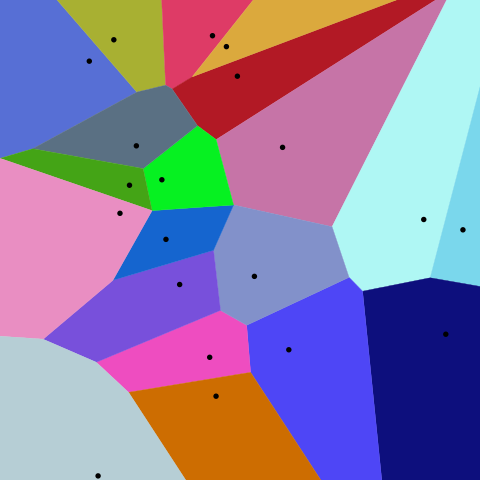
\includegraphics[width=0.5\textwidth]{./images/chapter3/Euclidean_Voronoi_diagram.png}
    \caption{Ευκλείδιο Διάγραμμα Voronoi}
    Πηγή: \href{https://en.wikipedia.org/wiki/Voronoi\_diagram}{https://en.wikipedia.org/wiki/Voronoi\_diagram}
    \label{fig:euclidean_voronoi}
\end{figure}

Το GVD είναι χρήσιμο στις ρομποτικές εφαρμογές, καθώς ο πραγματικός χώρος αναπαριστάται με μια διακριτή αναπαράσταση, τα OGM \ref{section:ogm}. Έτσι, μπορούν να υλοποιηθούν αλγόριθμοι εύρεσης του GVD του OGM ενός χώρου. Η πιο σημαντική περίπτωση είναι αυτή της χρήσης ως υποσύνολο σημείων όλα τα σημεία του OGM τα οποία αντιστοιχούν σε εμπόδια στον χώρο. Τότε σχηματίζεται ένα διάγραμμα που αποτελείται από τα πιο ασφαλή για την πλοήγηση του ρομποτικού οχήματος σημεία, καθώς αυτά απέχουν τις μέγιστες δυνατές αποστάσεις από τα γύρω εμπόδια. Ένα τέτοιο παράδειγμα είναι το \autoref{fig:gdv_example} \cite{wallgruen2009}. Το GVD ενός χώρου μπορεί να χρησιμοποιηθεί σε διάφορες εφαρμογές, όπως η εύρεση των πορτών των δωματίων \ref{subsection:find_door_nodes} ή η ταξινόμηση ενός υποχώρου σε δωμάτιο ή διάδρομο \ref{section:room_classification}.

\begin{figure}
    \centering
    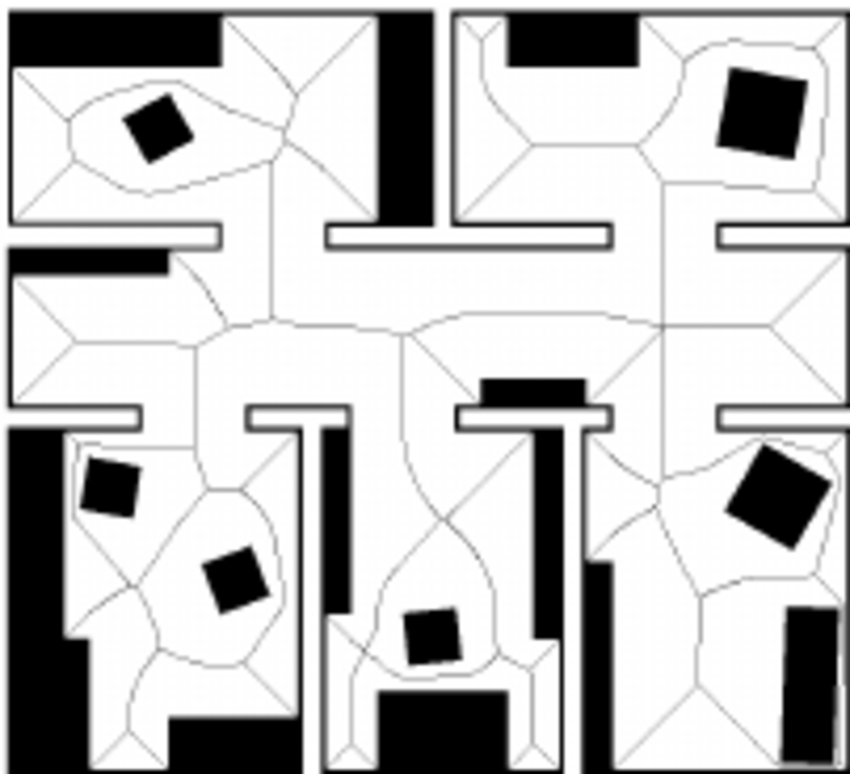
\includegraphics[width=0.5\textwidth]{./images/chapter3/gvd.png}
    \caption{GVD διδιάστατου χώρου}
    \label{fig:gdv_example}
\end{figure}
